%\newpage
\section{I-Maps}\label{sec:i-map}

This section studies the conditional independences in $G$. 

\subsection{Naive Bayes and Joint Probability}

First of all, we explain the difference between usual classification and Naive Bayes classifier. As shown in Figure~\ref{fig:naiveBayesPGM}, usual classification can be represented as a graphical model $G$ where the class label $Y$ receives incoming connections from the feature variables $X_1,...,X_n$. Therefore, $Y$ has a conditional probabilistic table $P(Y|X_1,...,X_n)$ and the feature variables $X_i$ has a marginal probability table $P(X_i)$. 
\begin{figure}[!htbp]
    \centering
    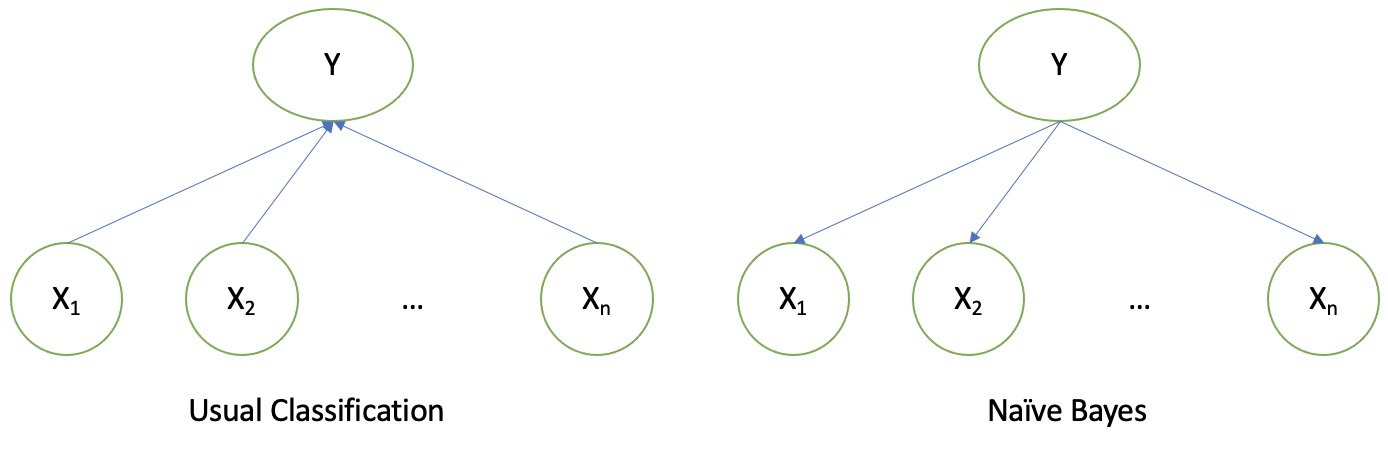
\includegraphics[width=0.9\textwidth]{images/graphical models/NaiveBayesPGM2.png}
    \caption{Naive Bayes as a probabilistic graphical model}
    \label{fig:naiveBayesPGM}
\end{figure}
However, for Naive Bayes classifier, it can be represented as another graphical model $G'$ where the label $Y$ has outgoing arrows to the feature variables $X_1,...,X_n$. Therefore, each feature variable $X_i$ has a conditional probability table $P(X_i|Y)$ and the class label has a marginal probability table $P(Y)$. As we explained earlier, for naive Bayes, we have 
%Intuitively, it says that, the random variable $Y$ conditionally depends on the other variables $X_1,...,X_n$, and once $Y$ is observed, $X_1,...,X_n$ are conditionally independent. We will explain this intuition later, and here we are interested to 
\begin{equation}
    P(X_1,...,X_n,Y)= P(Y)\prod_{i\in \{1..n\}}P(X_i|Y)
\end{equation}
That is, the joint probability is the product of probability tables for the nodes on the graph. Generalising the case for Naive Bayes classifier,  we conjecture that for 
 each probabilistic graphical model $G=({\cal V},{\cal E},P)$ represent the joint probability distribution between random variables, we may have  
\begin{equation}\label{equ:pajoint}
    P({\cal V})= \prod_{V\in {\cal V}}P(V|Pa(V))
\end{equation}
where $Pa(V)$ is the set of parent nodes of node $V$. Note that, we let $P(V|\emptyset) = P(V)$ when the node $V$ does not have incoming edges. 

\subsection{Independencies in a Distribution}\label{sec:distributionalindependencies}

Before proceeding to the conditional probabilities in $G$, we may need to know how to find conditional independencies from a joint probability. For this, Section~\ref{sec:indepandcondindep} has presented a few examples on how to do the calculation. 



 
\subsection{Markov Assumption}

In addition to the notation 
%We write 
$Pa(X)$ for the set of parents of a node $X$, we need $NonDesc(X)$ for the set of non-descendents of $X$. We have that 
\begin{tcolorbox}
each random variable $X$ is independent of its non-descendents, given its parents, i.e.,
\begin{equation}
    X\bot NonDesc(X) | Pa(X)
\end{equation}
\end{tcolorbox}
Intuitively, parents of a variable shield it from probabilistic influence. Once values of parents are  known, no influence of ancestors can be made. On the other hand, information about descendants can change beliefs about a node . 

For the running example in Figure~\ref{fig:graphicalmodel}, we have the following local conditional independences that can be read directly from the graph: 
\begin{equation}
    \begin{array}{lcl}
        I(G) &  = \{ & (Fog\bot Detected, Radar, Away, Stopped | Camera),  \\
         & & (Camera \bot Radar, Away) , \\
         & & (Radar \bot Camera, Fog) , \\
         & & (Detected \bot Away, Fog | Camera, Radar) , \\
         & & (Away  \bot Camera, Fog, Detected | Radar) , \\
         & & (Stopped \bot Fog, Camera, Radar | Detected, Away) \} \\
    \end{array}
\end{equation}
Intuitively, to understand $(Fog\bot Detected, Radar, Away, Stopped | Camera)$, we note  that, once we are able to observe the camera's result, the weather conditions such as $Fog$ can be directly obtained and are independent from other random variables. Moreover, to understand $(Camera \bot Radar, Away)$, we note that camera's precision -- as a quality of hardware --  is absolutely independent of both radar's result and whether or not the pedestrian is away. Other (conditional) independencies can be explained in a similar way. 

We remark that, the conditional independencies obtained through this way are local ones, and do not necessarily include all conditional independencies that can be inferred from the graph. In Section~\ref{sec:d-sep}, we will introduce a comprehensive method -- d-separation -- that is able to infer all possible conditional independencies from a graph. 

\subsection{I-Map of Graph and Factorisation of Joint Distribution}

Let $G$ be a graph associated with a set of independencies $I(G)$, and $P$ a probability distribution with a set of independencies $I(P)$. Note that, $I(P)$ can be obtained by the way shown in Section~\ref{sec:distributionalindependencies}. Then, we define 

\begin{definition}
$G$ is an I-Map of $P$ if $I(G)\subseteq I(P)$. 
\end{definition}

By this definition, I-Map requires that a joint
distribution $P$ can have more independencies than the graph $G$, but 
graph $G$ cannot mislead by containing independencies that do not exist in $P$. 

\begin{example}
Consider the joint probability table $P$ as in Table~\ref{tab:simpleJointProbability}, and the  three graphs in Figure~\ref{fig:simpleGs}. 
\begin{figure}[!htbp]
    \centering
    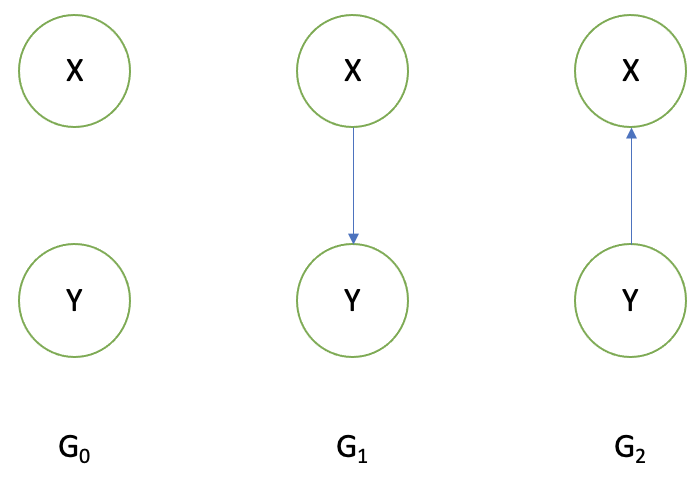
\includegraphics[width=0.4\textwidth]{images/graphical models/I-map/simpleGs.png}
    \caption{Three simple, two-node graphs}
    \label{fig:simpleGs}
\end{figure}
we note that $I(P)=\{X\bot Y\}$, $I(G_0)=\{X\bot Y\}$, and $I(G_1)=I(G_2)=\emptyset$. Therefore, all three graphs $G_0, G_1, G_2$ are I-maps of $P$. On the other hand, if consider  the joint probability table $P$ as in Table~\ref{tab:simpleJointProbability2}, we have that $I(P)=\emptyset$. Then, while $G_1$ and $ G_2$ are still I-maps of $P$, $G_0$ is not any more. 
\end{example}

In the following, we introduce the relationship between I-map and factorisation. Factorization is to write a mathematical object as a product of several, usually smaller or simpler, objects of the same kind. For example, in the Naive Bayes classifier, the joint distribution $P(X_1,...,X_n,Y)$ is rewritten as the production of $P(Y)$ and conditional probabilities $P(X_i|Y)$, where $P(Y)$ and $P(X_i|Y)$ are much smaller than $P(X_1,...,X_n,Y)$. For the graphical model in general, we have 

\begin{theorem}
If $G$ is an I-map of $P$, then 
\begin{equation}
    P(X_1,...,X_n) = \prod_{i=1}^n P(X_i|Pa(X_i))
\end{equation}
\end{theorem}
This justifies our conjecture at Equation (\ref{equ:pajoint}). 

\subsection{Perfect Map}

Similar as I-map, we may define D-map, which requires that $I(P)\subseteq I(G)$. The intersection of I-map and D-map leads to perfect map, which requires that the conditional independencies in $G$ and $P$. 
Interestingly, but not surprisingly, not all distributions $P$ over a given set of variables can be represented as a perfect map. 

